\scanpage{29}
structure locale de $X_j$ le long d'un $X_i$
(avec la stratification induite de type $I_{ij}$)
est ``cubique''
(coin de cube de dimension $n=\operatorname{card}S$)

\figure{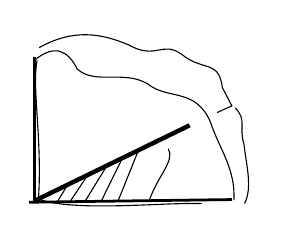
\begin{tikzpicture}[scale=0.85]
\draw[line width=1pt] (0,0)--(0,2.15);
\draw (0.06,0.02) .. controls (0.12,0.9) and (-0.04,1.7) .. (0.04,2.1);
\draw[line width=1pt] (-0.08,-0.02)--(2.95,0.02);
\draw (0.05,0.03) .. controls (0.6,-0.17) and (1.9,-0.02) .. (2.5,-0.04);
\draw (0,2.1) .. controls (0.3,2.35) and (0.5,2.25) .. (0.64,1.97)
.. controls (0.91,1.73) and (1.33,1.96) .. (1.69,1.75)
.. controls (2.0,1.5) and (2.4,1.7) .. (2.63,1.18)
.. controls (2.75,0.8) and (3.01,0.48) .. (2.98,0.01);
\draw (0.07,2.29) .. controls (0.59,2.58) and (1.01,2.5) .. (1.41,2.33)
.. controls (1.82,2.1) and (1.91,2.4) .. (2.2,2.19)
.. controls (2.54,1.92) and (2.75,2.12) .. (2.81,1.69)
--(2.95,1.42)--(2.73,1.32);
\draw (3.0,1.39) .. controls (3.18,1.21) and (3.05,1.1) .. (3.13,0.85)
.. controls (3.17,0.51) and (3.26,0.2) .. (3.14,-0.04);
\draw[line width=1.6pt] (0,0)--(2.32,1.13);
\draw (0.35,0)--(0.49,0.23);
\draw (0.54,0)--(0.8,0.39);
\draw (0.76,0)--(1.08,0.52);
\draw (1.0,0)--(1.32,0.65);
\draw (1.25,0)--(1.56,0.77);
\draw (1.72,0.02) .. controls (1.86,0.4) and (2.1,0.6) .. (2.0,0.78);
\end{tikzpicture}}

La \deleted{condition c)} impliquent que si $j'$ est
un prédécesseur de $j$, et si $k\in I$ est $\le j$
mais non $\unsure{\le|<}j'$, et s'il existe
un $i$ majoré par $k$ et $j'$, \uline{alors}
$k'=\operatorname{Inf}(k,j')$ existe, et $k'$ est
un prédécesseur de $k$.

\diagram{\begin{tikzcd}[column sep=small,row sep=small]
& j' \arrow[r,leftrightarrow,"\mathrm{préd}"'] \arrow[d,phantom,"{\unsure{\downarrow}}" description] & j \arrow[d,phantom,"{\unsure{\downarrow}}" description] \\
& k' \arrow[r,leftrightarrow] & k \\
i \arrow[uur,hook] \arrow[urr,hook] & &
\end{tikzcd}}

(Il suffit de voir que dans
un ens. ordonné de la forme $\mathcal P(\sigma)$,
les inf existent (c'est l'intersection) et si
$j'\subset j=j'\amalg\{\alpha\}$, et $k\in j$ mais non $k\subset j'$,
alors \deleted{$\unsure{k\ne k'}$} $k=k'\amalg\{\alpha\}$ avec $k'=k\cap j'$, \ldots)
\margin{$\sigma$ ens fini}

Ceci posé, considérons le diagramme
\diagram{\begin{tikzcd}
X_{j'} \arrow[r,hook] & X_j \\
X_{k'} \arrow[u] \arrow[r,hook] & X_k \arrow[u]
\end{tikzcd}}
où les flèches verticales, par l'hyp. $\unsure{1^\circ|a)}$,
sont des plongements bordants. Ceci posé, on
voit \inserted{(par b,c)} que \deleted{$X_k\longrightarrow X_{\unsure{j}}$}
$(X_k,X_{k'})\mathbin{-}(X_j,X_{j'})$
\margin{28}
